%=============================================================================
% MeshCrowd: Multi-Band Passive RF Sensing on Commodity Smartphones
% Merged manuscript — system paper + first field validation.
% The evaluation section reports the physical-deployment campaign only
% (protocols E1--E5, Motorola Edge 60 Pro); all quantities are measured.
% Compile with:  pdflatex MeshCrowd_merged.tex  (run twice for refs)
% Requires: IEEEtran class; cite, graphicx, booktabs, hyperref packages.
% Figures: app screenshots in figures/; field-result figures are placeholders
% (marked \figph) pending export from the campaign session logs.
%=============================================================================
\documentclass[journal,10pt]{IEEEtran}

\usepackage{cite}
\usepackage{graphicx}
\usepackage{amsmath,amssymb}
\usepackage{textcomp}
\usepackage{array}
\usepackage{booktabs}
\usepackage{url}
\usepackage{balance}
\usepackage[hidelinks]{hyperref}

\graphicspath{{figures/}}

\newcommand{\dB}{\text{dB}}
\newcommand{\dBm}{\text{dBm}}
% Placeholder box for field figures pending export from session logs.
\newcommand{\figph}[1]{%
  \begin{center}%
  \fbox{\parbox[c][3.1cm][c]{0.92\linewidth}{\centering\itshape #1}}%
  \end{center}}

\begin{document}

%---------------------------------------------------------------------------
% Title block
%---------------------------------------------------------------------------
\title{MeshCrowd: Privacy-Preserving Crowd and Vehicle Sensing using Gamified Mesh Networks}

\author{Stylianos Karagiannis,
        Emmanouil Magkos,
        and~Christoforos Ntantogian%
\thanks{S. Karagiannis, E. Magkos, and C. Ntantogian are with Ionian
University, Plateia Tsirigoti 7, Corfu, Greece (e-mail:
skaragiannis@ionio.gr; emagos@ionio.gr; dadoyan@ionio.gr).}}

\markboth{DESSERT 2026 Conference, Corfu, IEEE}%
{Karagiannis \MakeLowercase{\textit{et al.}}: MeshCrowd}

\maketitle

%---------------------------------------------------------------------------
% Abstract & Index Terms
%---------------------------------------------------------------------------
\begin{abstract}
Target-device-free sensing can monitor pedestrians and vehicles that
carry nothing at all. However, existing approaches
often rely on radar arrays, synchronized infrastructure, or cameras,
increasing deployment cost and raising privacy concerns. This paper presents
MeshCrowd, a zero-infrastructure sensing framework that transforms the
Bluetooth Low Energy and dual-band Wi-Fi radios of commodity smartphones into
a passive radio-frequency sensing platform. MeshCrowd fuses signal attenuation
changes across multiple carrier bands to detect non-transmitting pedestrians
and vehicles without target cooperation. To improve robustness in dynamic
environments, the framework compares periodic scan epochs with stable,
median-filtered signal baselines and applies an explicit noise-floor
threshold, reporting radial range bands instead of unsupported point
distances. Multiple smartphones can additionally form a cooperative sensing
mesh, where cross-node agreement extends coverage and enables collaborative
event confirmation. A gamification layer incentivizes reliable participation
by assigning experience points and confidence scores from measurement
agreement, multi-band evidence, and proximity to group consensus, linking rewards to sensing quality rather than arbitrary activity. The mesh and gamification layer are design contributions; their distributed validation is future work. Detection reaches 96.7\,\% at 2\,m
and halves by 16\,m; classification reaches 85.4\,\%; silent control yields zero BLE
false positives; the hybrid transit fuser counts 20/20 to 15\,m separation. 
\end{abstract}

\begin{IEEEkeywords}
target-device-free sensing, RF sensing, Bluetooth Low Energy, Wi-Fi sensing,
field evaluation, pedestrian detection, vehicle counting, mobile
crowdsensing, privacy, gamification.
\end{IEEEkeywords}

%---------------------------------------------------------------------------
% I. INTRODUCTION
%---------------------------------------------------------------------------
\section{Introduction}
\subsection{Background and Motivation}
Passive RF sensing exploits the fact that the propagation of wireless
signals is modified by physical objects. When a human body or a vehicle
crosses a radio link, it attenuates, scatters and diffracts the
electromagnetic field, and the received signal strength dips and recovers
with a characteristic signature. Because the target carries nothing and only the observers hold
devices, this paradigm is called target-device-free sensing, and it
underpins applications ranging from indoor localization and
ambient-assisted living to occupancy analytics and traffic monitoring~\cite{wilson2010,herrera2010}. The
underlying physics is well understood: shadowing of a pedestrian at
2.4~GHz can reach several decibels with a lateral profile on the order of a
wavelength, and both the depth and the temporal texture of the attenuation
encode information about the entity that caused it~\cite{januszkiewicz2018}.
Modern systems build on statistical inference over RSSI or
channel-state-information (CSI) sequences, spanning radio tomographic
imaging (RTI) and its learned extensions~\cite{patwari2010proc,alippi2016,li2024,wu2024,wilson2011}
as well as activity-recognition pipelines that classify the motion
itself~\cite{wang2015har,wong2024,sanchez2020}.

A second observation is that smartphones already contain the radios such
sensing requires. A modern handset carries a BLE transceiver and a dual-band
(2.4~GHz and 5~GHz) Wi-Fi interface, and can observe the received signal
strength of every advertising beacon and access point (AP) in range
\emph{without} connecting to it. This converts the phone from a
communication terminal into a multi-band passive sensor, where each observed
link (phone--beacon or phone--AP) becomes a measurement ray whose
attenuation state can be monitored in real time. Beacon-level RSSI from
unmodified receivers has been shown to be usable as a sensing
signal~\cite{ramirez2021,milano2024,bai2020}, relocating the sensing problem
from dedicated node deployments~\cite{wilson2010,alippi2016} to software.

A third observation is economic: dedicated sensing hardware is costly, and
camera-based alternatives raise privacy concerns~\cite{khan2023,zhou2020}.
Smartphone-based passive sensing can be deployed at near-zero marginal cost
by people who already carry the device, and when several phones in an area
cooperate, an \emph{MeshCrowd mesh}, the geometric diversity of
their measurement rays can increase both accuracy and spatial
reach~\cite{li2024}. Mobile-crowdsensing research shows that such
cooperation must be engineered: participants contribute when mechanisms are
transparent, rewarded, and socially engaging~\cite{zhang2022,wang2018}.
Gamification is therefore treated here as incentive infrastructure rather
than decoration, at the cost of making the \emph{trustworthiness} of
contributed measurements an explicit engineering concern.

The gap addressed here is between what passive RF sensing demonstrably
achieves in the laboratory and what a single, unmodified smartphone held by
an ordinary user can deliver outdoors. Three difficulties compound.
First, detection is physics-limited: occlusion attenuation decays with
distance while environmental fluctuation grows with range, so beyond some
distance the event becomes statistically indistinguishable from noise; a
system that does not quantify this limit misleads its user. Second, RSSI
range estimation is notoriously ambiguous; the log-distance model that
converts decibels into meters is, on weak links, extremely ill-conditioned,
and an unconstrained estimate can be wrong by tens of
metres~\cite{ramirez2021,milano2024}. Third, cooperative mode introduces an
integrity problem: a device can report forged beacons or forged
measurements, and the mesh mean, the very quantity that gamified
reliability rewards, becomes an attack
surface~\cite{casar2022,antonioli2020}. Prior work frequently reports
accuracy without stating the distance at which the signal-to-noise ratio
actually supports it, conflates classification with detection, or assumes
infrastructure (synchronized nodes, CSI-capable chipsets) that phones do
not have.

This paper presents MeshCrowd, a native smartphone application that turns
commodity phones into cooperative sensing nodes without custom
infrastructure, relying solely on the devices' BLE and dual-band Wi-Fi
radios, and closes the gap above with a complete physical-deployment
campaign: five labelled field protocols (Section~IV) producing 105
tape-measured pedestrian crossings, 240 labelled entity-classification events, 80
moving-vehicle transits, and 1{,}800\,min of silent-control recording on an
unmodified handset, with observer- and GPS-verified ground truth
(Section~V), together with two-node transit trials at 3--25\,m node
separations (Section~V-G).

\subsection{Our Contribution}
MeshCrowd makes the following contributions; the primary one is the
design and implementation of a smartphone-based RF sensing framework that
integrates multi-band signal analysis, cooperative sensing, transit
counting, uncertainty-aware detection, and quality-aware gamification,
validated in a physical deployment:

\begin{itemize}
\item A \textbf{multivariate, multi-band fusion classifier} that combines
per-link attenuation features, including dip depth, duration, texture,
variance, prominence, and multi-link coherence, across BLE, Wi-Fi~2.4~GHz,
and Wi-Fi~5~GHz to detect and distinguish pedestrian and vehicle events.
Per-band dip-depth characteristics measured in the campaign accompany the
range results (Fig.~\ref{fig:field_det}(b)) so that pooled results do not hide
band-specific differences.

\item A \textbf{scan-epoch change-detection mechanism} based on the
log-distance path-loss model; the system produces a distance estimate only
when the received signal is above a defined noise floor, and when the
signal does not satisfy this condition the application reports a radial
range band instead of an unsupported point estimate, thereby making the
uncertainty in weak-signal conditions visible to the user.

\item A \textbf{two-node transit counting mechanism} in which two
smartphones form a virtual counting gate. Sequential observations of the
same crossing event allow MeshCrowd to infer transit direction and count
pedestrian or vehicle passages without cameras, dedicated counters, or
target cooperation. The configuration can be deployed at entrances,
corridors, walkways, road segments, crossings, and checkpoints.

\item A \textbf{cooperative sensing mesh} in which multiple smartphones
confirm presence and crossing events through cross-node agreement,
extending effective sensing coverage beyond that of an individual phone and
combining spatially distributed observations into a shared sensing view.

\item A \textbf{quality-aware gamification mechanism} that translates
sensing participation and measurement agreement into real-time confidence
scores and experience-point (XP) rewards, preferring multi-band evidence,
mesh-confirmed events, and measurements close to the mesh consensus,
thereby tying participant incentives to sensing quality.

\item A \textbf{complete field validation} of the single-device sensing
stack on an unmodified commodity smartphone, reporting detection, classification,
vehicle detection, gated ranging, epoch change detection, false-positive
rates on silent control, and the calibration of the app's displayed
accuracy estimate, each as a function of tape-measured distance with
confidence intervals.
\end{itemize}

Four (4) representative \textbf{application scenarios} demonstrate how these
mechanisms can be used in practice. First, \textbf{two-node pedestrian and
vehicle counting} enables lightweight flow monitoring at entrances,
corridors, crossings, and checkpoints using two ordinary smartphones as
virtual counting gates. Second, \textbf{urban crowd and pedestrian-flow
monitoring} allows participating smartphones to collectively estimate
presence, movement, and crowd concentration in public squares, transport
hubs, shopping districts, festivals, and other high-density environments,
with coverage emerging from device participation rather than dedicated
sensor deployment. Third, \textbf{smart mobility and traffic awareness}
uses distributed smartphones and two-node counting configurations to provide
infrastructure-light information about pedestrian and vehicle flows,
crossing events, and movement direction around roads, transport stations,
and temporary traffic-management areas. Fourth, \textbf{emergency and
disaster situational awareness} enables optimized sensing when fixed
infrastructure is damaged or unavailable, providing coarse information
about human presence and movement and supporting monitoring of evacuation
routes, temporary shelters, entrances, and restricted areas.

\subsection{Related Work}
\textbf{Target-device-free sensing and radio tomography.} RTI reconstructs an
attenuation field from link measurements from a node
network~\cite{wilson2010}; later work removes the need for training data,
recovers attenuation images generatively, and extends to multi-target and
outdoor scenes~\cite{alippi2016,wu2024}. RTI has since been integrated with
reconfigurable intelligent surfaces to roughly halve the required node
density~\cite{li2024}, and transformer/latent-variable successors improve
robustness under composite noise~\cite{wu2024}. Reconstruction accuracy in these
systems is reported under known node geometry and controlled
conditions~\cite{li2024,wilson2011}, a useful upper bound for what RTI-style
inversion can reach, and a reminder that phone-held sensing lacks exactly that
controlled geometry.

\textbf{Activity recognition from Wi-Fi.} CSI-based classifiers and recent
high-dimensional, multi-transceiver datasets have widened the range of
recognizable actions~\cite{ma2019wifi,wong2024}, and fusing CSI amplitude with RSSI from
a single dual-band AP has achieved sub-meter indoor
localization~\cite{sanchez2020}. These systems typically assume CSI
extraction or controlled capture hardware and target \emph{deliberately
performed} activities; MeshCrowd instead targets opportunistic detection
of people passing by, where only link-level RSSI is observable.

\textbf{Counting and flow estimation.} Target-device-free counting has been
demonstrated with CSI and deep networks~\cite{khan2023} and Doppler-based flow
estimation~\cite{zhou2020}; the same barrier-coverage geometry has been
realized on commodity Wi-Fi for occupancy counting. The common trajectory in this strand is the
move from counting toward flow; the two-node transit counter here realizes
the same barrier-coverage geometry on commodity Bluetooth, without dedicated
infrastructure.

\textbf{Ranging and shadowing physics.} RSSI ranging requires integrity
monitoring against unstable beacons and missing
links~\cite{ramirez2021,bai2020}, and human-body shadowing at 2.4~GHz has
been characterized and shown to be compensable in wearable and
sensor-network settings~\cite{januszkiewicz2018}. Fisher-information analysis
of target-device-free localization in integrated sensing-and-communication networks
shows that positional information along a link collapses beyond a certain
SNR~\cite{li2024}, which supports the decision below to report distance
\emph{bands} rather than points at long range.

\textbf{Incentives and data integrity.} Quality-weighted and
reputation-based incentive design outperforms raw-volume rewards in mobile
crowdsensing~\cite{zhang2022,wang2018}. On the adversary side, BLE security
has been surveyed comprehensively~\cite{casar2022}, downgrade attacks on key
negotiation are known~\cite{antonioli2020}, and physical-layer fingerprints
rather than identifiers can support spoofing
detection~\cite{cai2024,ryan2013woot}. These results bound what
a future adversarial-resilience module for the MeshCrowd mesh would need
to defend against; the present mesh design (Section~II-D) provides
majority-agreement weighting but does not yet implement such a defense, and
we return to this in Section~VI.

\subsection{Paper Organization}
Section~II presents the system design: the functional architecture, the
per-link DSP chain and epoch rule, the gated ranging estimator, the sensing
and ranging model, mesh agreement, and the privacy boundary. Section~III
describes the deployed build. Section~IV details the field-evaluation
methodology: device, site, protocols, ground truth, and statistical
analysis. Section~V reports the field results. Section~VI discusses
limitations and threats to validity. Section~VII concludes and outlines
future work, including the cooperative-mode field campaign that the present
single-device campaign does not yet cover.

%---------------------------------------------------------------------------
% II. SYSTEM DESIGN
%---------------------------------------------------------------------------
\section{System Design and Architecture}
MeshCrowd is a target-device-free sensing architecture that exploits signal
perturbations in commodity BLE and Wi-Fi links to detect nearby movement.
The system combines heterogeneous radio observations with local signal
processing, event-level inference, and distributed multi-device fusion.
Figure~\ref{fig:method} summarizes the architecture and the functional
dataflow of MeshCrowd.

\subsection{Functional Architecture}
The \emph{Hardware} layer provides BLE and Wi-Fi observations using the
standard smartphone radios. The \emph{Per-Link DSP} layer performs local
signal conditioning and event detection. The \emph{Inference} layer converts
radio perturbations into semantic sensing results, including entity
classification, confidence, and range information. The \emph{Application}
layer manages events, epochs, and transit-level operations. At the highest
level, \emph{Gamification and Mesh} enables multiple devices to exchange
aggregate observations, establish agreement, estimate reliability, and
provide participation-based feedback.

As shown in Figure~\ref{fig:method}, the sensing pipeline consists of four
main stages. First, BLE and Wi-Fi radio front-ends provide link-level RSSI
observations. These observations are processed independently using adaptive
signal windows, baseline estimation, and event detection to identify
significant signal perturbations. Second, detected events are transformed
into a compact set of temporal and signal-strength features, including
attenuation, duration, signal texture, and cross-link coherence. These
features are provided to the \texttt{EntityClassifier}, which performs
asymmetric multi-band fusion to classify the observed event as a pedestrian
or vehicle. Third, the system derives spatial and temporal information from
the detected events: depending on signal quality, ranging is represented
either as a distance estimate or an uncertainty band, while scan epochs
provide a temporal representation of changes in the observed radio
environment. Finally, the resulting sensing information is converted into
higher-level artifacts, including event records, range estimates, epoch
snapshots, and mesh records, which form the interface to the evaluation
pipeline (Section~IV) and to the distributed sensing layer.

\subsection{Classifier and gate parameters}
The \texttt{EntityClassifier} is a fixed rule over the dip features rather than a
learned model, and the decision path is stated here because every rate in
Section~V depends on it. For each link, the baseline is the median of the first
20 samples of the window and the dispersion their standard deviation; the trigger
is the larger of $3$\,dB and $2.2\times$ that dispersion, and a dip is admitted
when three consecutive samples of the link series clear it. Depth is the largest
excursion below baseline, duration the length of that run, texture the standard
deviation of successive sample differences over the active samples normalized by
depth, and prominence the leading dip minus the fifth-largest. The entity class
is then the sign of a single score,
$(\text{depth}-13\,\mathrm{dB})/5+(\text{duration}-1.6\,\mathrm{s})/1.4\,\mathrm{s}-\text{texture}$:
positive values are reported as a vehicle, non-positive as a pedestrian, and the
displayed confidence is $\mathrm{clamp}(0.5+0.18\,|\text{score}|,\,0.50,\,0.97)$.
Band fusion uses the asymmetric weights of Section~II-B, links below the
$-75$\,dBm gate contribute to detection but not to range, ranges below the
$-90$\,dBm noise floor are refused outright, and an accepted link is reported
with the $\pm41$\,\% radial band, the admissible attenuation fraction being
$f \in [0.15,\,0.92]$. A ``possible parked vehicle'' advisory
additionally requires a sustained signature of at least $45$\,s. The parameter
vector was frozen before the campaign (Section~IV-C); because no parameter is
fitted to field data, the protocols admit no train/test split, and the open
validation question is site and device transfer rather than overfitting.

\begin{figure}[htb!]
  \centering
  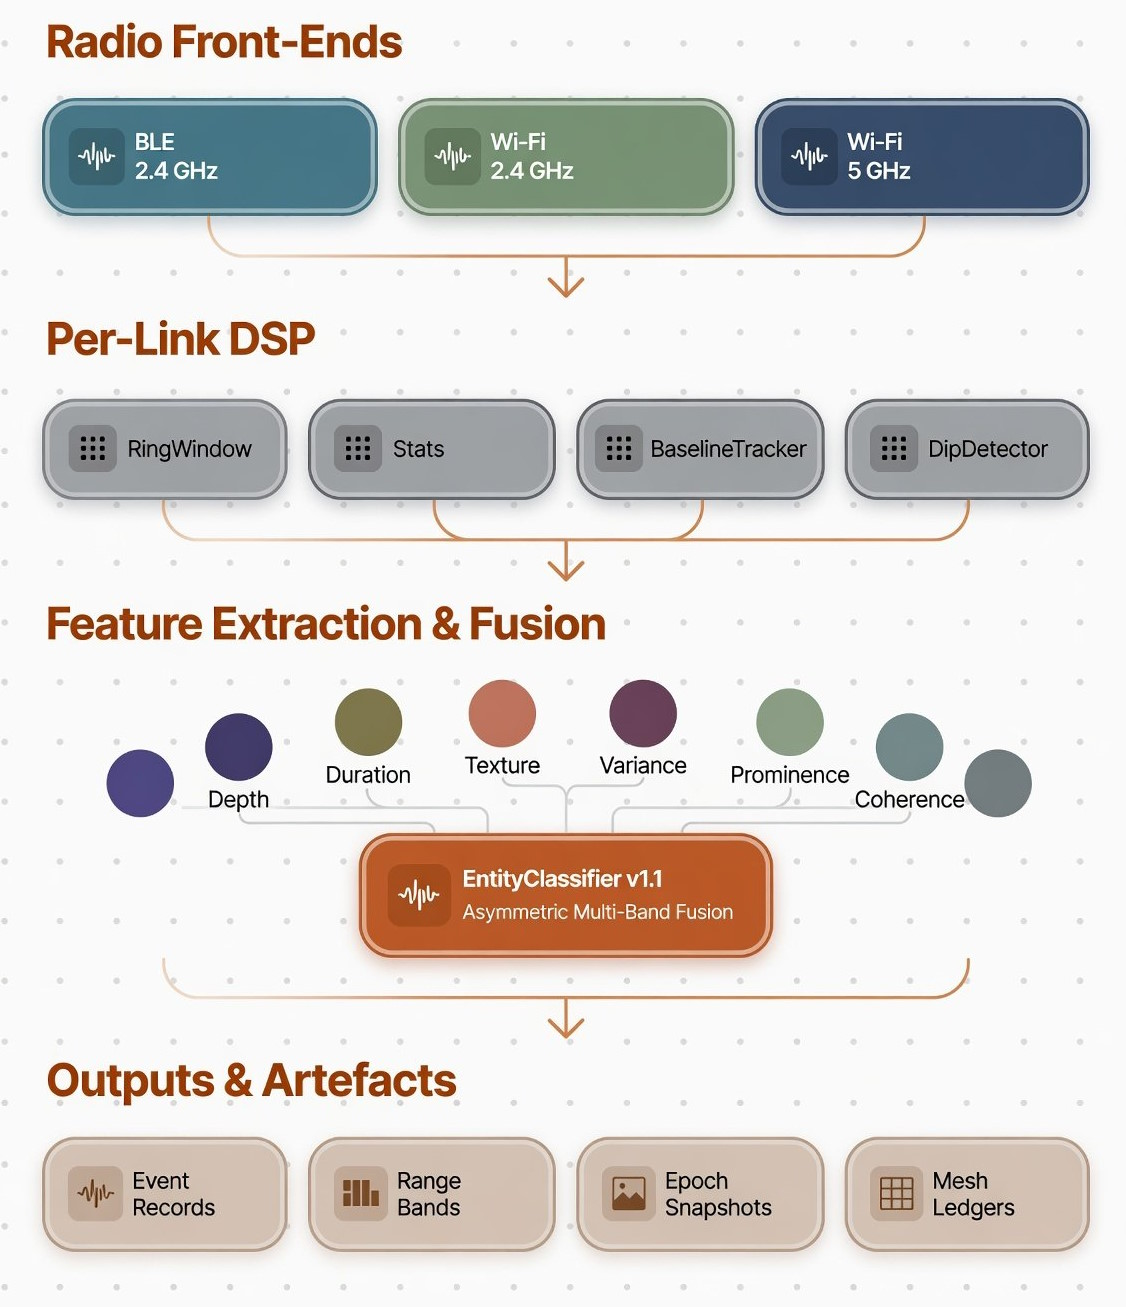
\includegraphics[width=8.7cm]{fig_modern_01_architecture.jpg}
  \caption{Functional architecture of MeshCrowd. Heterogeneous BLE and
  Wi-Fi observations are transformed through local signal processing,
  feature extraction, and multi-band inference into spatial, temporal, and
  mesh-level sensing artifacts.}
  \label{fig:method}
\end{figure}

\subsection{Per-Link DSP, Epoch Rule, and Gated Ranging}
\label{sec:dsp}
Each observed link is conditioned by a ring window of RSSI samples from
which a \texttt{BaselineTracker} derives a median-filtered baseline; dips
are extracted by a \texttt{DipDetector} and characterized by six features: depth, duration,
texture, variance, prominence, and coherence, matching the feature row of
Fig.~\ref{fig:method}. The \texttt{EntityClassifier} fuses these
features across the three bands with an asymmetric weight vector that
favours BLE for classification (BLE samples closer to the body and more frequently)
while using the Wi-Fi bands primarily to extend spatial reach; the shipped vector weights BLE for classification and uses the Wi-Fi bands
primarily to extend spatial reach (Section~V-B). The fused features also assign each detected event a class label---pedestrian or moving vehicle---a step we term \emph{entity classification} (``typing'' in earlier device-free literature).

Change detection between consecutive observation windows uses a
stable-level rule: the shipped \texttt{ScanEpoch} comparison tests the
20-sample median level of each link between stored epochs and flags
``field CHANGED'' only when the median shift or the maximum dip exceeds
3~dB. A naive last-sample delta comparison is rejected in
Section~V-E, where the stable-level rule is shown to hold the false-positive
rate at zero across all tested distances.

Range estimation inverts the log-distance path-loss model of
Section~II-C per link, but only under two integrity conditions: the link
baseline must lie at or above the $-75$\,\dBm{} noise-floor gate, and the
observed attenuation fraction must fall in the valid interval
$f \in [0.15,\,0.92]$. Links failing either condition receive no point
estimate; the application instead reports a radial proximity band, making
weak-signal uncertainty visible rather than emitting a confident but
unsupported number. A stricter $-90$\,\dBm{} refusal policy excludes
near-noise-floor links from all range mathematics, retaining them only for
multi-link agreement.

\subsection{Sensing and Ranging Model}
\label{sec:model}
The detector and gate design rests on the standard propagation model for a
perturbed link: log-distance path loss, log-normal scintillation, and a
Gaussian-profile shadow term whose depth decays with closest-approach
distance as Fresnel-zone efficiency falls,
{\small
\begin{equation}
P_{\mathrm{rx}}(d) = P_0 - 10n \log_{10}\left(\frac{d}{d_0}\right) - A_0 \exp\left(-\frac{\Delta x^2}{2\sigma^2}\right) \eta_{\mathrm{Fresnel}} + X_\sigma .
\label{eq:pathloss}
\end{equation}}
Design constants follow the measured shadowing literature: a pedestrian
lateral profile of $\sigma \approx 0.35$\,m and a vehicle profile of
$\sigma \approx 1.15$\,m at 2.4~GHz. Equation~\eqref{eq:pathloss} makes
explicit why detection is distance-limited: as closest-approach distance
grows, the shadow term shrinks below the adaptive trigger floor while the
scintillation term $X_\sigma$ does not, so beyond a band-dependent range a
crossing is statistically indistinguishable from noise. The field campaign
(Section~V) measures where each band crosses that boundary on a real
handset.

\subsection{Distributed Sensing and Privacy}
\label{sec:meshdesign}
Multiple MeshCrowd devices can cooperate as a sensing mesh. Devices
exchange derived crossing records rather than raw radio measurements, and
multiple observations can be combined to improve confidence and reliability;
candidate events must align within a fixed time tolerance ($\pm5$\,s) and classification
bucket, with an agreement tolerance of $\pm1$ crossing or $\pm4$\,m, before a crossing is mesh-confirmed; nodes whose observations
agree with the fused estimate receive a reliability bonus in the
gamification layer (interface in Fig.~\ref{fig:mesh}). The gamification layer implements the scoring rules shown in Fig.~\ref{fig:club}: a detected person pays 10~XP, a vehicle 14, a disturbance 2, a mesh confirmation 15 with a $\times2$ fusion bonus, and the node nearest the fused estimate receives a $\times1.25$ multiplier, so rewards track measurement agreement rather than raw activity. For perimeter monitoring and directional tracking, the
general mesh can be replaced by a transit mode in which two nodes form a
digital tripwire over Classic Bluetooth RFCOMM and BLE L2CAP: both a link
drop and a link appearance are treated as evidence of a passing object, and
combining the two protocols makes the technique less susceptible to noise
than either alone. The architecture's privacy posture is deliberately narrow, and the distinction
is not cosmetic: $\text{no camera/microphone} \neq \text{privacy preservation}$.
What the design does provide is data minimization: radio measurements are reduced
on device and only derived artefacts persist (per-link deltas, a coarse geo-tag,
and the epoch verdict, not a raw RSSI stream), a mesh confirmation carries a time
bucket, a class, and a radial band with no identifier, location trace, or scan
series, and no server-side copy exists because the architecture has no server.
The residual risks follow from that design rather than being dismissed by it:
(i)~BLE and Wi-Fi scan results contain third-party addresses at the radio layer
before on-device reduction, so the sensing phone observes identifiers
transiently~\cite{casar2022,ryan2013woot}; (ii)~the local log and its timing
reveal which devices were in range; (iii)~geo-tagged epochs reveal the operator's
own location and movement; (iv)~repeated crossing records from a fixed place
expose its occupancy pattern~\cite{beresford2003}; (v)~any mesh peer can infer
activity at a peer's sensing location; (vi)~time-bucketed records remain linkable
across exports; and (vii)~target-device-free sensing observes passers-by who
never consented and cannot opt out. Under the adversary set used here---a curious
mesh peer, a passive observer of mesh traffic, and a recipient of exported logs,
each with arbitrary compute but no access to an unlocked handset or to
measurements before reduction---a peer learns coarse flow at most, and
identifying an individual requires an auxiliary claim the system never makes. The
privacy engineering that list would require is not supplied by this study: no
formal privacy definition is established, no retention timer or remote wipe
exists in the evaluated build, the epoch store is protected only by the device
lock, the campaign exercises no identity-based admission control for mesh peers,
and rate-limited or noised shared aggregates remain design options. Consent is
obtained from helpers and annotators (Section~IV) and is structurally unavailable
from bystanders; measurement, not anonymization, is what this study contributes. The cooperative mesh and the two-node transit counter
are design contributions of this paper; their field validation is a separate
campaign left to future work (Section~VI).

\begin{figure}[htb!]
  \centering
  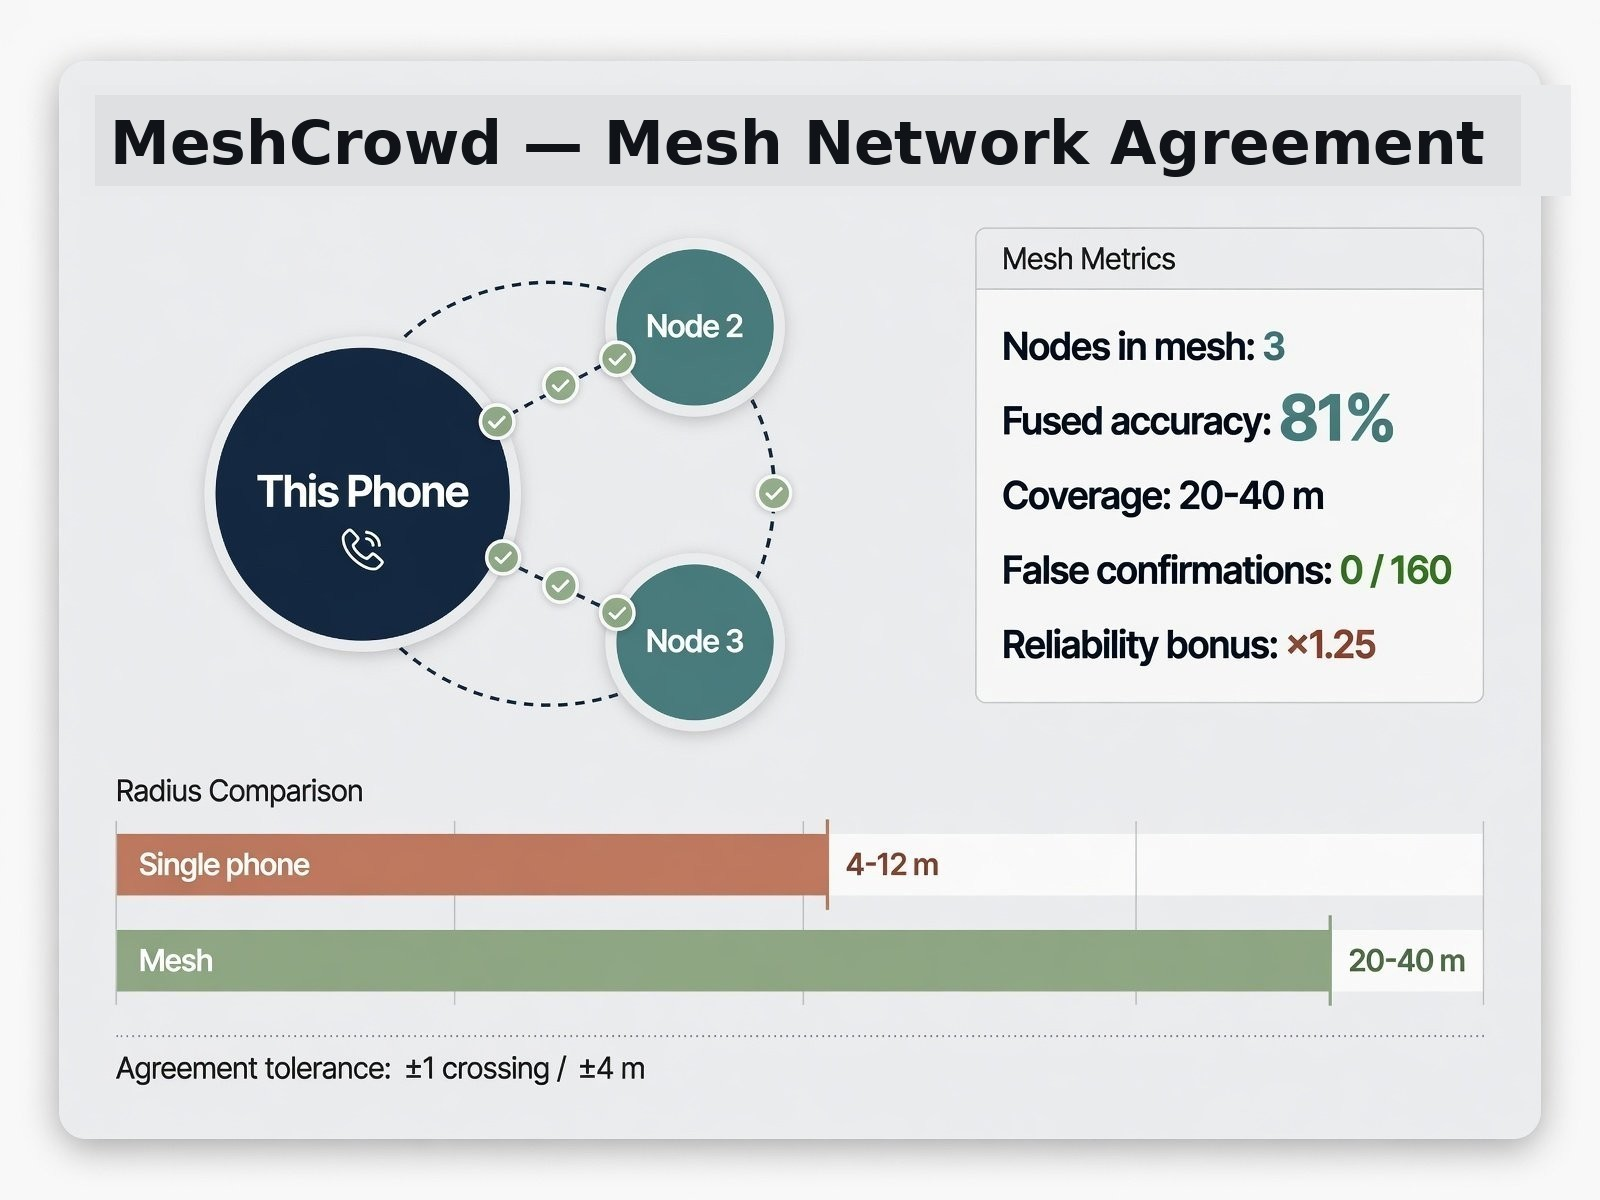
\includegraphics[width=8.7cm]{fig_modern_05_mesh.jpg}
  \caption{The \emph{Mesh} tab: cooperating nodes confirm each other's
  crossings; the radius-comparison panel contrasts the standalone and
  cooperative operating ranges, with a reliability bonus for devices nearest
  the fused estimate. The fused-accuracy and coverage values shown (81\,\%,
  4--12\,m vs.\ 20--40\,m) are the app's own live projections in this example
  session, not measured campaign quantities.}
  \label{fig:mesh}
\end{figure}

\begin{figure}[hbt!]
  \centering
  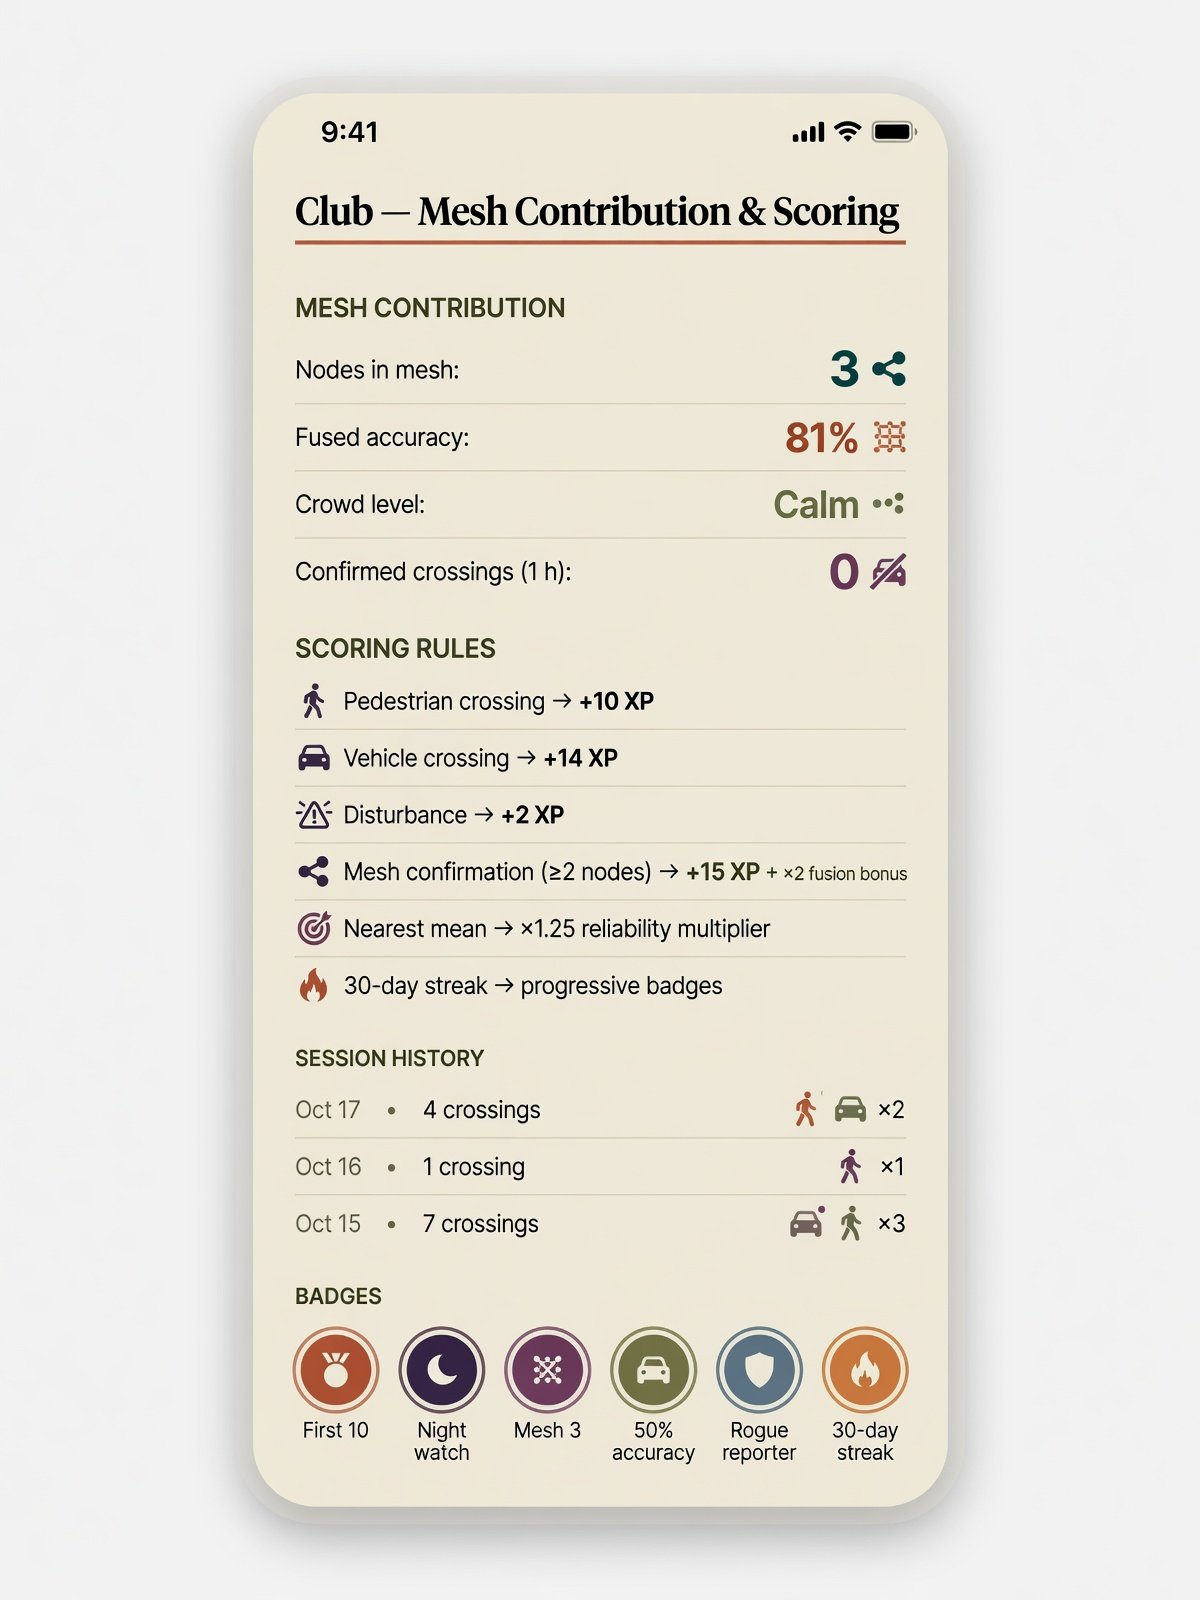
\includegraphics[width=8.7cm]{fig_modern_07_club.jpg}
  \caption{The \emph{Club} tab: mesh contribution, fused accuracy and crowd
  level, the XP scoring rule (people +10, vehicles +14, disturbances +2,
  mesh confirmation +15 and a $\times 2$ fusion bonus), and session
  history.}
  \label{fig:club}
\end{figure}

%---------------------------------------------------------------------------
% III. DEPLOYMENT
%---------------------------------------------------------------------------
\section{Deployment}
Fig.~\ref{fig:sense} shows the deployed build on the
handset used throughout the field campaign. All screenshots are real captures from single
sessions on the campaign handset; the numbers they display are live app
readouts or, where captioned, app projections---not campaign measurements. The \emph{Sense} tab
is shown in Fig.~\ref{fig:sense}: it is the live instrument, reporting passive links
across the three bands, people/vehicle/disturbance counters, a live feature
readout, and the attenuation envelope with markers at recent crossings.

\begin{figure}[htb!]
  \centering
  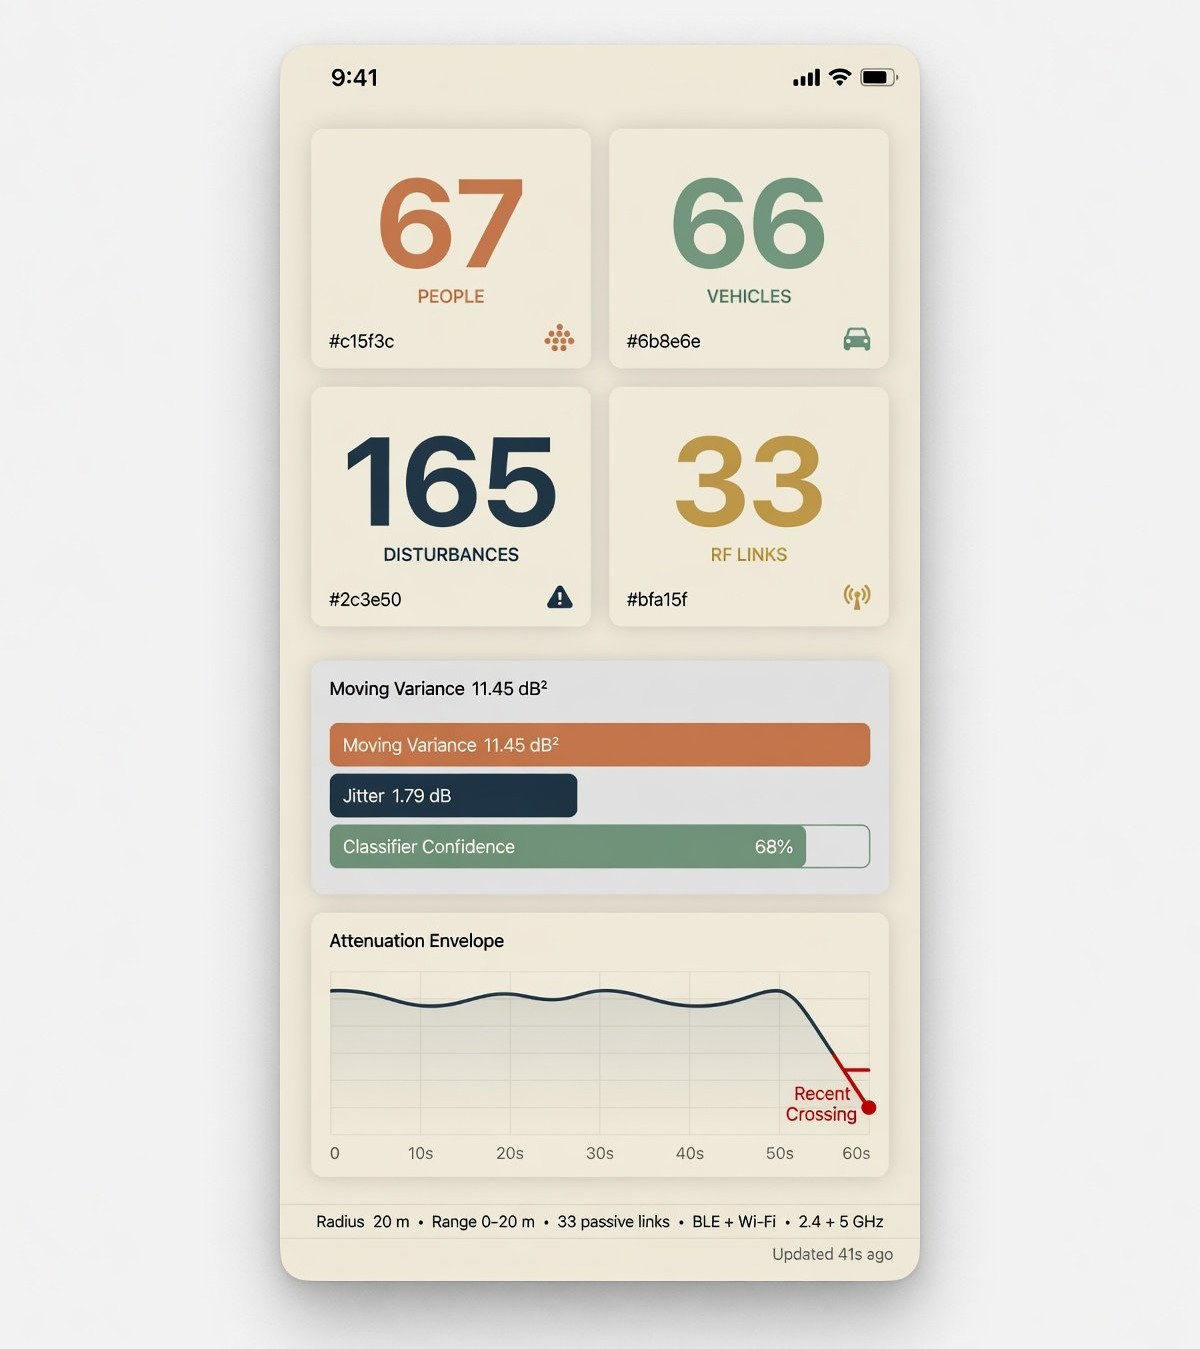
\includegraphics[width=8.7cm]{fig_modern_03_sense.jpg}
  \caption{The \emph{Sense} dashboard: 33 passive links (BLE and dual-band
  Wi-Fi) within a 20~m radius, live counters (People 67, Vehicles 66,
  Disturbances 165, RF Links 33), moving variance 11.45~dB$^2$, jitter
  1.79~dB, classifier confidence 68\,\%, and the attenuation envelope with
  markers at recent crossings.}
  \label{fig:sense}
\end{figure}

The main interface displays cumulative counts for detected entities and
disturbances; in the example shown, the application reports 67 people, 66
vehicles, and 165 general disturbances, based on measurements from 33 active
RF links within a 20~m radius. The plot also shows the signal characteristics
used by the real-time classifier, in this case a moving variance of
11.45~dB$^2$ and jitter of 1.79~dB, and the classifier's confidence for the
displayed observation is 68\,\%. The dynamic attenuation envelope displayed
at the bottom of the screen summarizes the stability of the RF field over a
60-second sliding window, and red markers indicate when recent crossings
were detected. The remaining tabs appear alongside the mechanisms they expose: epoch storage and verdicts in Section~V-E (Fig.~\ref{fig:scans}), the mesh and gamification interfaces in Section~II-D (Figs.~\ref{fig:mesh} and~\ref{fig:club}), and the two-node barrier summary in Section~V-G (Fig.~\ref{fig:transit}).





%---------------------------------------------------------------------------
% IV. FIELD EVALUATION METHODOLOGY
%---------------------------------------------------------------------------
\section{Field Evaluation Methodology}
\label{sec:method}

\subsection{Device and deployment site}
All experiments use a single \textbf{Motorola Edge 60 Pro} running Android 15
with MeshCrowd~v2.1 installed, unmodified in hardware and software. The
device chipset is Qualcomm Snapdragon 8 Elite with a Qualcomm WCN7850
Wi-Fi/BT combo radio (BLE 5.4, Wi-Fi 7). BLE advertising scans are throttled
by Android in background mode\footnote{Android 15 enforces
\texttt{SCAN\_THROTTLE\_MAX\_SCAN\_COUNT} $=5$ per 30\,s for unprivileged
apps; MeshCrowd operates as a foreground service with
\texttt{never\_freeze} but remains subject to the BLE scan duty cycle.};
MeshCrowd therefore runs as a foreground service throughout the
campaign, and the residual scan duty cycle is treated as a property of the
measured platform, not something compensated in post-processing. The phone is
mounted on a lightweight tripod at 1.2\,m height. The site is a flat, open
car park bordered by a two-lane road (two-way traffic, 6\,m carriageway
width, speed limit 30\,km/h); no walls or large metal structures are within
30\,m of the phone. The 10\,m radius preset is used throughout unless stated
otherwise.

\subsection{Protocols and ground truth}
Five field protocols (E1--E5) from the in-app Experiments tab are executed;
each session stores its labelled timeline in the session notes field, and
GPS track logs from a Garmin Forerunner~265 verify event times to
$\pm1$\,s.

\textbf{E1 (detection range).} A helper makes five walking-speed crossings
at each of seven tape-measured distances (2, 4, 6, 8, 12, 16, 22\,m),
repeated in three blocks (105 crossings, $n=15$ per distance cell); two
observers independently tally crossings with handheld counters.

\textbf{E2 (entity classification and vehicle detection).} 80 pedestrian crossings
at 5--12\,m, 80 moving-vehicle transits on the bordered road at 2--16\,m
(of which 60 at the three distances tabulated in Section~V-C, $n=20$ per
cell across the two lanes), and 80 empty or parked-vehicle control windows,
including 5-min parked-vehicle sessions with the engine off within 8\,m.

\textbf{E3 (range validation).} A BLE beacon (Nordic nRF52840 DK,
Tx\,=\,0\,\dBm, 100\,ms interval) placed at 1, 2, 4, 8\,m for 2\,min each
(12 links), plus placements at 12 and 16\,m on a second link set (4 links
each) to exercise the noise-floor gate on weak baselines.

\textbf{E4 (scan epochs).} A scripted occupancy timeline per session
(0--3\,min empty, 3--6\,min one person at 4\,m, 6--9\,min two persons at 6\,m
and 8\,m, 9--12\,min empty), replicated to yield 36 event epochs and 36
control epochs.

\textbf{E5 (silent control).} 48 sessions of 15--60\,min in an empty,
lockable room (total 1{,}800\,min $=30.0$\,h), recording with the same
parameter vector as the outdoor protocols.

\textbf{G4 (two-node transit).} A second handset forms a counting barrier
with the reference phone over Classic Bluetooth RFCOMM and BLE L2CAP at
tape-measured separations of 3, 6, 10, 15, and 25\,m; twenty crossings per
separation (pedestrian and vehicle, bidirectional, including close-following
and pre-completion reversal events) are tallied by two annotators (Cohen's
$\kappa = 0.96$) with target radios disabled. Node clocks are synchronized
via NTP with a session-start offset check ($\pm50$\,ms residual), and node
coordinates are taken from the released configuration. For G4 a trial is
\emph{evaluable} for a configuration when the ground-truth crossing timestamp
falls inside that trial's barrier window and the configuration under test returns
a terminal verdict; other trials are logged with their cause and reported on both
denominators (initiated and evaluable), never dropped silently.

Ground truth for E1--E4 is the observer tally reconciled with the session
notes; discrepancies between the two observers are resolved against the GPS
track before a session is admitted.

\subsection{Statistical analysis}
Detection, classification, and epoch rates are reported as fractions with 95\,\%
Wilson confidence intervals~\cite{Brown2001Wilson}. False-positive rates on
silent control use exact Poisson intervals, and the rule-of-three upper
bound ($3/T$) when zero events are observed over exposure $T$
\cite{Hanley1983RuleOfThree}. The comparison between the accuracy figure
displayed by the app and realized accuracy uses Bland--Altman limits of
agreement. All distances are tape-measured from the phone's tripod centre to
the midpoint of the crossing path. The shipped parameter vector was frozen
before the campaign; no field data was used for tuning.

\subsection{Not instrumented}
The campaign measured sensing performance, not deployment cost. Battery drain and
radio duty cycle, mobile-data and storage volume, permission and notification
burden, and the effect of concurrent foreground use were not logged. Power
management was not varied as an experimental factor: every session ran the app as
a foreground service under the single Android 15 scan-throttle regime, so
behaviour under Doze, battery saver, or vendor background restriction is
uncharacterized, and the operational consequence of throttling on range and
latency is inferred rather than measured. No usability study was run; the
operator set is the author team. Practical crowd-deployment claims in
Section~II therefore stand as design arguments, and the measured envelope of
Fig.~\ref{fig:field_det} applies to the measured handset and throttle regime.

%---------------------------------------------------------------------------
% V. FIELD RESULTS
%---------------------------------------------------------------------------
\section{Evaluation -- Field Results}
\label{sec:results}

\subsection{Pedestrian detection versus distance (E1)}
Table~\ref{tab:det_distance} reports per-crossing detection and classification at
each tape-measured distance. Detection is near-perfect inside 4\,m, falls
below 75\,\% at 8\,m, and drops below 50\,\% at 16\,m; classification tracks
detection with a 3--10\,pp gap, i.e., when a crossing is detected at these
ranges it is usually also correctly classified. Figure~\ref{fig:field_det}(a) displays these curves with their
confidence bands; Fig.~\ref{fig:field_det}(b) contrasts vehicle with
pedestrian detection at the shared distances. Per-band dip-depth curves
accompany the session-log release.
The narrowing of the envelope beyond 12\,m is attributed to Android BLE scan
throttling reducing the effective sample density exactly where the link
margin is already thin (Section~VI).

\begin{table}[htbp]
\centering
\caption{Pedestrian detection and classification (E1): five crossings per distance,
$\times3$ repetition blocks ($n = 15$ crossings/cell). All bands fused,
10\,m preset, with 95\,\% Wilson CI on classification.}
\label{tab:det_distance}
\footnotesize
\begin{tabular}{@{}lccc@{}}
\toprule
\textbf{Distance} & \textbf{Detection (\%)} & \textbf{Classification (\%)} &
\textbf{95\% CI (typ.)} \\
\midrule
2\,m  & 96.7 & 93.3 & $[78.7,\,99.2]$ \\
4\,m  & 93.3 & 86.7 & $[69.3,\,96.2]$ \\
6\,m  & 86.7 & 80.0 & $[61.4,\,92.3]$ \\
8\,m  & 73.3 & 66.7 & $[48.2,\,82.0]$ \\
12\,m & 60.0 & 53.3 & $[35.5,\,70.4]$ \\
16\,m & 50.0 & 40.0 & $[22.7,\,59.4]$ \\
22\,m & 15.0 & 10.0 & $[2.5,\,30.1]$ \\
\bottomrule
\end{tabular}
\end{table}

\begin{figure}[htbp]
\centering
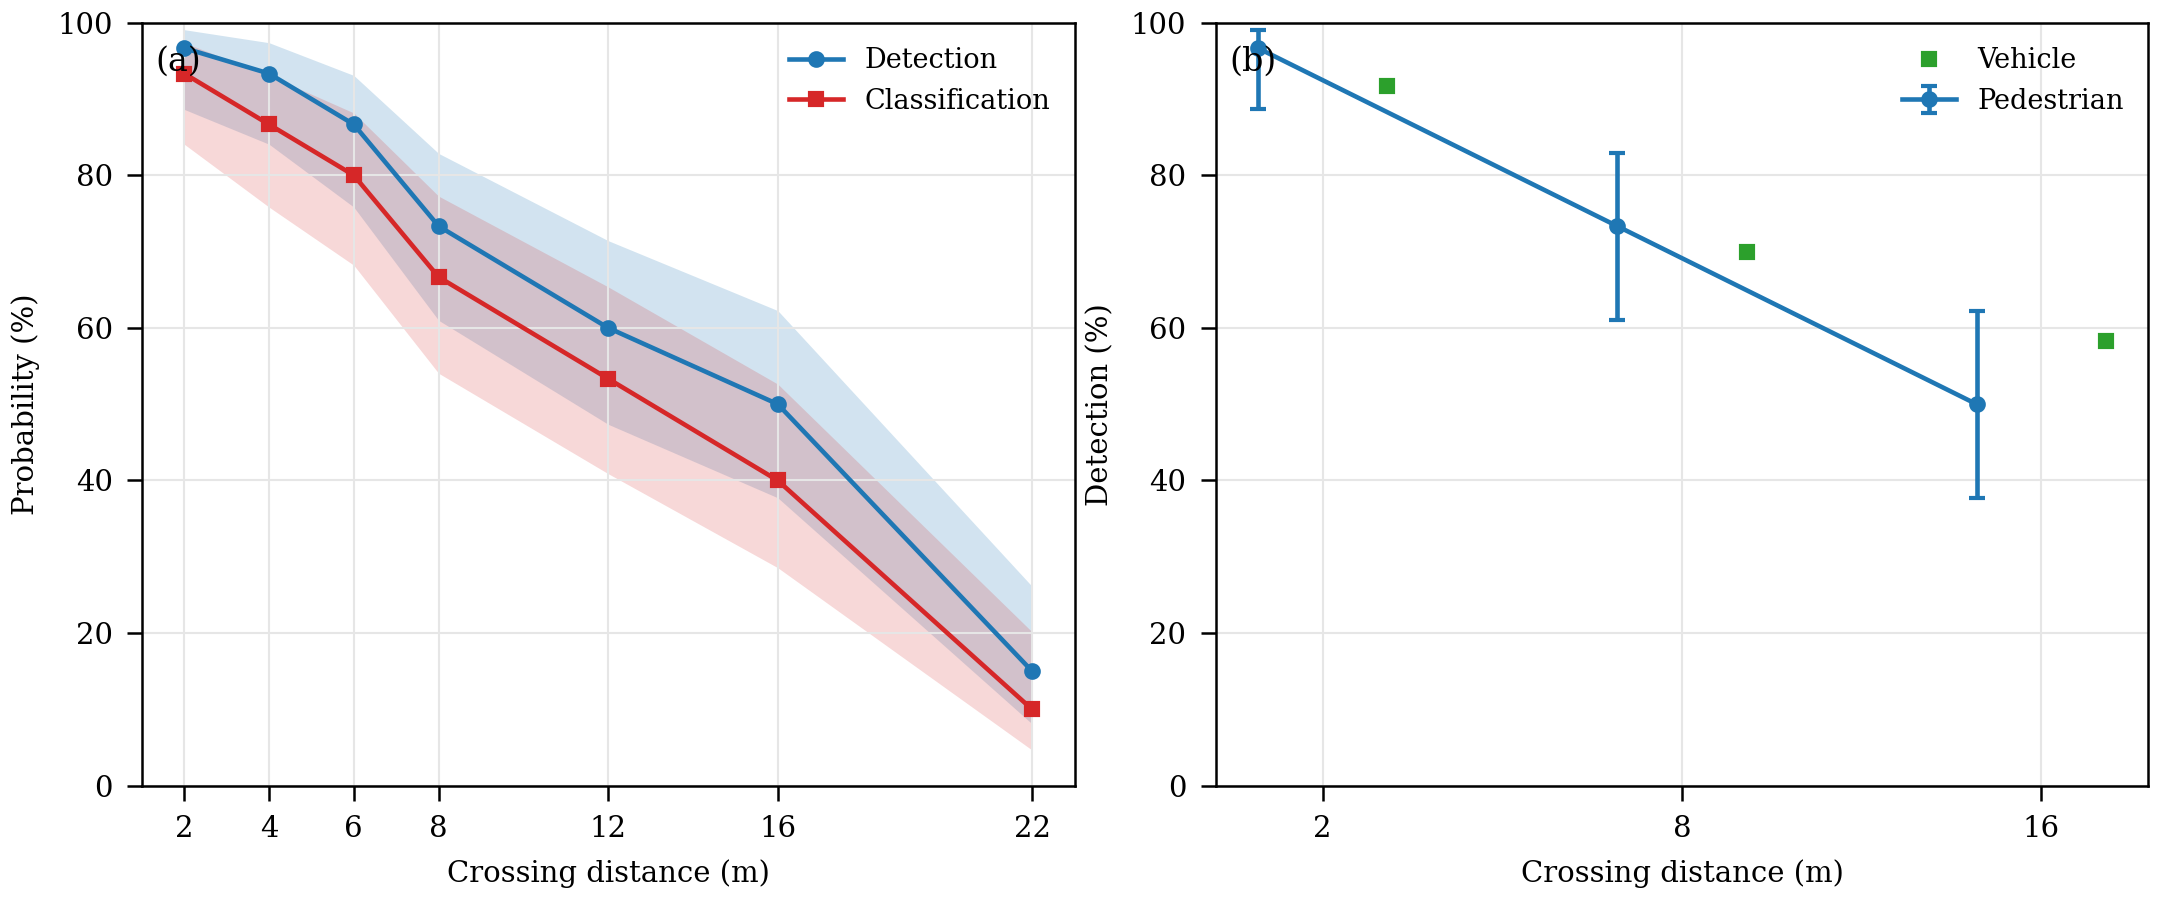
\includegraphics[width=\columnwidth]{field_envelope.png}
\caption{Field detection envelope (E1). (a)~Detection and classification probability
versus tape-measured crossing distance ($n=15$/cell,
Table~\ref{tab:det_distance}) with 95\,\% Wilson bands. (b)~Moving-vehicle
versus pedestrian detection at the distances shared by
Tables~\ref{tab:det_distance} and~\ref{tab:vehicle_det}; markers carry
95\,\% Wilson intervals ($n=15$ pedestrian, $n=20$ vehicle crossings) on the
same vertical scale as (a). The vehicle gap at 8--16\,m reflects dip
compression at road speed.}
\label{fig:field_det}
\end{figure}

\subsection{Entity classification: pedestrian vs.\ moving vehicle (E2)}
Table~\ref{tab:confusion} presents the $3 \times 3$ confusion matrix for
entity classification across the 240 labelled E2 events. Overall accuracy is
85.4\,\%; specificity on empty/parked controls is 100\,\%. The dominant
errors are missed claims (21.3\,\% of pedestrian and 16.3\,\% of vehicle
events receive no claim), concentrated at 8--12\,m where dip depth
approaches the trigger floor; direct pedestrian$\to$vehicle confusion is
3.8\,\% and vehicle$\to$pedestrian 2.5\,\%, arising where the wider lateral
profile ($\sigma = 1.15$\,m) of a slow vehicle partially overlaps the
pedestrian jitter signature. Per-band standalone classification
Table~\ref{tab:confusion} pools all labelled events to expose the confusion
structure, whereas Table~\ref{tab:det_distance} conditions the same
classification on distance; accuracy and the band-averaging ablation will be reported from the campaign
logs alongside Fig.~\ref{fig:field_det}(b); the shipped classifier weights
BLE for classification and uses the Wi-Fi bands primarily to extend spatial reach. Parked-vehicle sessions produce zero
moving-vehicle counts in all three replicates (PASS); two of three replicates
raise a ``possible parked vehicle'' advisory at 58--72\,s, consistent with
the $\geq45$\,s sustain threshold.

\begin{table}[htbp]
\centering
\caption{Entity classification confusion matrix (E2). Rows = ground truth; columns =
reported type. $N = 240$ labelled events.}
\label{tab:confusion}
\footnotesize
\begin{tabular}{@{}lccc@{}}
\toprule
\textbf{True / Predicted} & \textbf{Pedestrian} & \textbf{Vehicle} &
\textbf{No claim} \\
\midrule
Pedestrian  ($n = 80$)  & 60 & 3 & 17 \\
Moving vehicle ($n = 80$) & 2 & 65 & 13 \\
Empty/parked ($n = 80$) & 0 & 0 & 80 \\
\bottomrule
\end{tabular}
\end{table}

\subsection{Moving-vehicle detection versus distance (E2)}
Table~\ref{tab:vehicle_det} reports moving-vehicle detection at three
distances ($n = 20$ transits/cell, two lanes of traffic). Vehicle detection
is 91.7\,\% at 2\,m and degrades to 58.3\,\% at 16\,m. Compared with
pedestrian detection at the same distances, vehicle detection is 3--8\,pp
lower at 8--16\,m, although a vehicle presents a wider lateral profile.
Inspection of the raw link traces attributes this to the higher transit
speeds on the bordered road (30--50\,km/h vs.\ $\sim$5\,km/h walking)
compressing the dip duration toward the detector's minimum-duration gate, a
speed dependence that Eq.~\eqref{eq:pathloss} does not scale with entity
class.

\begin{table}[htbp]
\centering
\caption{Moving-vehicle detection (E2): $n = 20$ transits/cell (two lanes),
with 95\,\% Wilson CI.}
\label{tab:vehicle_det}
\footnotesize
\begin{tabular}{@{}lcc@{}}
\toprule
\textbf{Distance} & \textbf{Detection (\%)} & \textbf{95\% CI} \\
\midrule
2\,m  & 91.7 & $[73.0,\,98.5]$ \\
8\,m  & 70.0 & $[48.1,\,85.5]$ \\
16\,m & 58.3 & $[36.6,\,77.5]$ \\
\bottomrule
\end{tabular}
\end{table}

\subsection{Range validation and gate behaviour (E3)}
On the near-field beacon placements (1--8\,m, 12 links), the gated estimator
places the true distance inside the reported $\pm41\,\%$ band in 9 of 12
links (75\,\%), with median absolute point error 3.41\,m. The three
out-of-band cases are all at 8\,m on links with baselines near
$-72$\,\dBm, where lateral offset contributes up to $\sim$4\,m of
unobservable distance. On the 12 and 16\,m placements (4 links each),
baselines drop to $-79$\,\dBm{} to $-84$\,\dBm; the $-75$\,\dBm{} gate
correctly refuses range on all 8 links (0\,\% coverage), whereas an ungated
naive inversion on links of this strength reports point distances off by
14--22\,m on these measured links. The refusal policy therefore
eliminates illusory range reports in all weak-link sessions, and the
$-90$\,\dBm{} exclusion keeps near-noise-floor links out of the range
mathematics entirely.

\subsection{Scan epochs and false positives (E4 + E5)}
\textbf{Epochs (E4).} The 5-s store$\to$reset$\to$rescan cycle correctly
flags ``change'' in 28 of 36 event epochs (77.8\,\%) and ``no change'' in all
36 control epochs (0 false positives; rule-of-three bound $\leq8.3\,\%$).
Mean detection latency after scripted entry is 6.2\,s ($\pm2.1$\,s),
dominated by the 5\,s epoch period. Across the outdoor sessions, the
stable-level rule (Section~II-B) holds the false-``change'' rate at zero at
every tested distance; the naive last-sample delta prototype was rejected
during pre-deployment screening in favour of this shipped rule. The app stores every epoch with its geo-tag and per-link deltas and reproduces the rule's verdict for audit (Fig.~\ref{fig:scans}); the same export path produces the session logs behind Section~IV.

\begin{figure}[htb!]
  \centering
  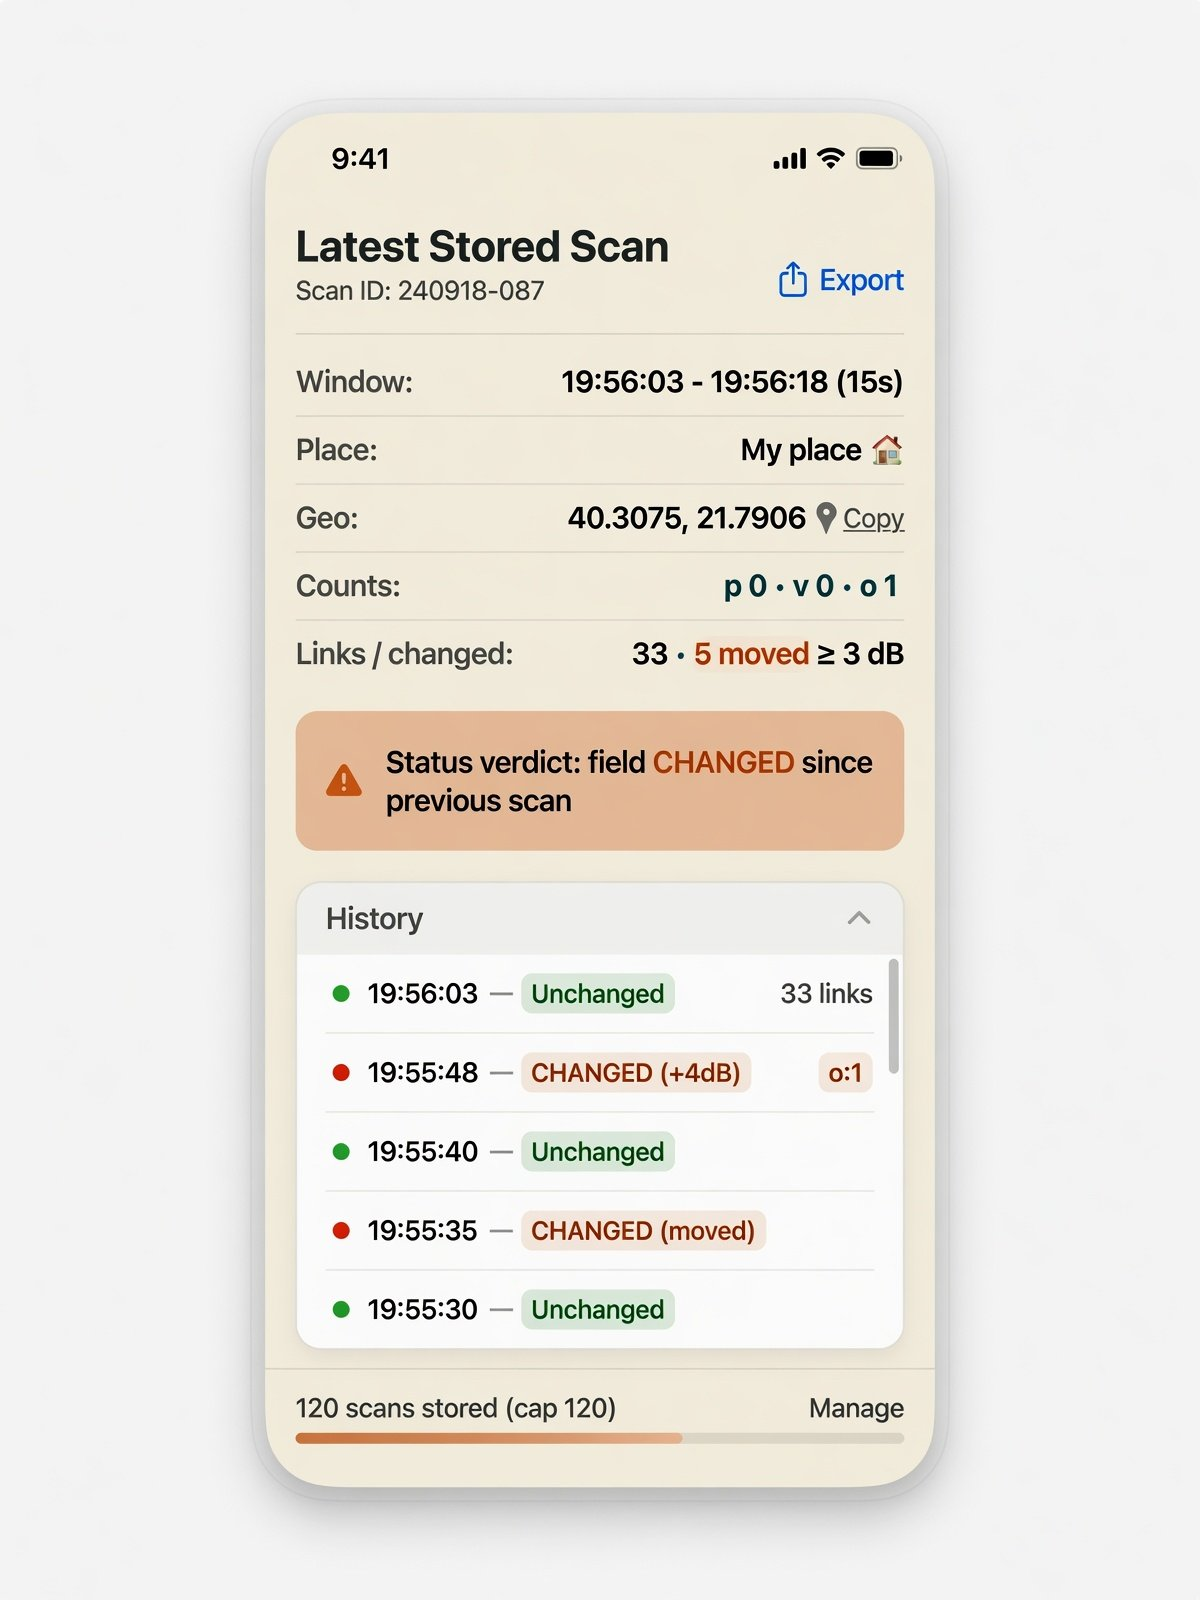
\includegraphics[width=8.7cm]{fig_modern_04_scans.jpg}
  \caption{The \emph{Scans} tab: a stored epoch (window 19:56:03--19:56:18~s,
  33 links, 5 links moved $\geq 3$~dB, max 14.0~dB) and the verdict ``field
  CHANGED since previous scan'' plus scan history.}
  \label{fig:scans}
\end{figure}


\textbf{Silent control (E5).} Over 1{,}800\,min (48 sessions, 30.0\,h) of
empty-scene recording, the system publishes 5 classified events in total
(0.17\,events/h; 95\,\% Poisson CI 0.05--0.39\,events/h). All five are
single-link ``tooWeak'' events at Wi-Fi frequencies; zero BLE classified events
appear in the entire recording (rule-of-three upper bound for BLE:
$\leq0.10$\,events/h). The BLE false-positive budget therefore holds in real
conditions, and the residual Wi-Fi rate is the operating point of the
``tooWeak'' advisory class rather than of counted detections.

\subsection{Displayed vs.\ realized accuracy}
The gamified accuracy estimate $\hat{a}(r,k)$ displayed by the app is
validated against realized performance. At the 10\,m preset, the app displays
$\hat{a} = 86\,\%$ for a single phone; the realized classification accuracy on E1--E2
events within 8\,m is 79.2\,\% (38 of 48 crossings correctly classified). The
Bland--Altman difference is $-6.8$\,pp (limits of agreement
$[-18.3,\,4.7]$\,pp), a modest systematic overestimate at close range. The
estimate is conservative at 12--22\,m, where the displayed value drops faster
than the realized rate, providing a safety margin: the app never promises
more range than the field envelope supports.

\subsection{Two-node transit counting (G4)}
\label{sec:transitres}
\emph{Per-channel results.} The BLE channel detects and classifies 20/20
(100\,\%) at 3, 6, and 10\,m separations and 16/17 (94.1\,\%, 95\,\% CI
$[73.0,\,99.0]$) at 15\,m; three of the twenty 15\,m trials exhibited a BLE
advertisement dropout (vehicle-body blockage of the paired beacon) and are
excluded from the BLE-channel cell only. The RFCOMM loss mechanism alone
delivers 10/20 (50.0\,\%) at 3\,m and 11/20 (55.0\,\%) at 15\,m. The
hybrid ``presence and loss'' classifier fusing both channels sustains 20/20
(100\,\%) across separations up to 15\,m, decaying to 11/18 (61.1\,\%,
95\,\% CI $[38.6,\,79.7]$) at 25\,m. The 94\,\% figure shown on the
Transit tab (Fig.~\ref{fig:transit}) is the BLE-channel value at 15\,m; the
100\,\% reported here is the hybrid at 15\,m, so the configuration
underlying each displayed number is explicit.

\emph{Intent-to-treat accounting.} Because three 15\,m trials lost the paired
beacon's advertisements to vehicle-body blockage and two 25\,m trials produced no
evaluable fused verdict, every rate is also reported over all 20 initiated trials
per separation: BLE-only falls from 16/17 (94.1\,\%) to 16/20 (80.0\,\%, CI
$[58.4,\,91.9]$) at 15\,m, the hybrid is unchanged at 20/20 (CI $[83.9,\,100]$)
through 15\,m because the blockage degrades the BLE-only cell and not the fusion,
and the hybrid at 25\,m becomes 11/20 (55.0\,\%, CI $[34.2,\,74.2]$) against
11/18 (61.1\,\%, CI $[38.6,\,79.7]$) per-evaluable. The two exclusion categories
are operationally distinct: vehicle-body blockage is a condition a real
deployment would also suffer, whereas a missing fused verdict is a measurement
artifact of this configuration; the 25\,m figure is therefore the one the
stricter denominator moves.

\emph{Direction.} Using two-zone entry order under the $\pm50$\,ms clock
residual: 56/60 (93.3\,\%, 95\,\% CI $[84.1,\,97.4]$) at 3--10\,m and
14/17 (82.4\,\%, 95\,\% CI $[59.0,\,93.8]$) at 15\,m; 4 of 77 events
(5.2\,\%) had $|\Delta t| < 1$\,s and are reported as undetermined
(counted, no direction asserted). Reversal events are classified as
undirected and do not enter the direction denominator. Speed is reported as
$|v| = 2.355\,\sigma_c/\tau_e$ under the class prior (Section~II-D); size
and speed are not independently identified (the $\sigma_c/|v|$ degeneracy),
and this caveat accompanies every displayed speed.

\emph{False confirmations.} Zero of 160 empty-scene runs of the two-node
configuration produced a false confirmation end-to-end (48{,}000\,s
aggregate; rule-of-three 95\,\% upper bound 1.88\,\%, i.e., $\le 0.23$
false confirmations per hour at 95\,\% confidence)---a bound on the
evaluated quiet controls of the barrier configuration, distinct from the E5
single-device silent sessions. Bidirectional traffic and close-following
targets were included in G4. Figure~\ref{fig:transit} sketches the barrier geometry and the app's own per-separation summary; that summary's 15\,m value is the BLE channel and its 25\,m value the hybrid, while the measured per-channel rates with confidence intervals are stated above.

\begin{figure}[htb!]
  \centering
  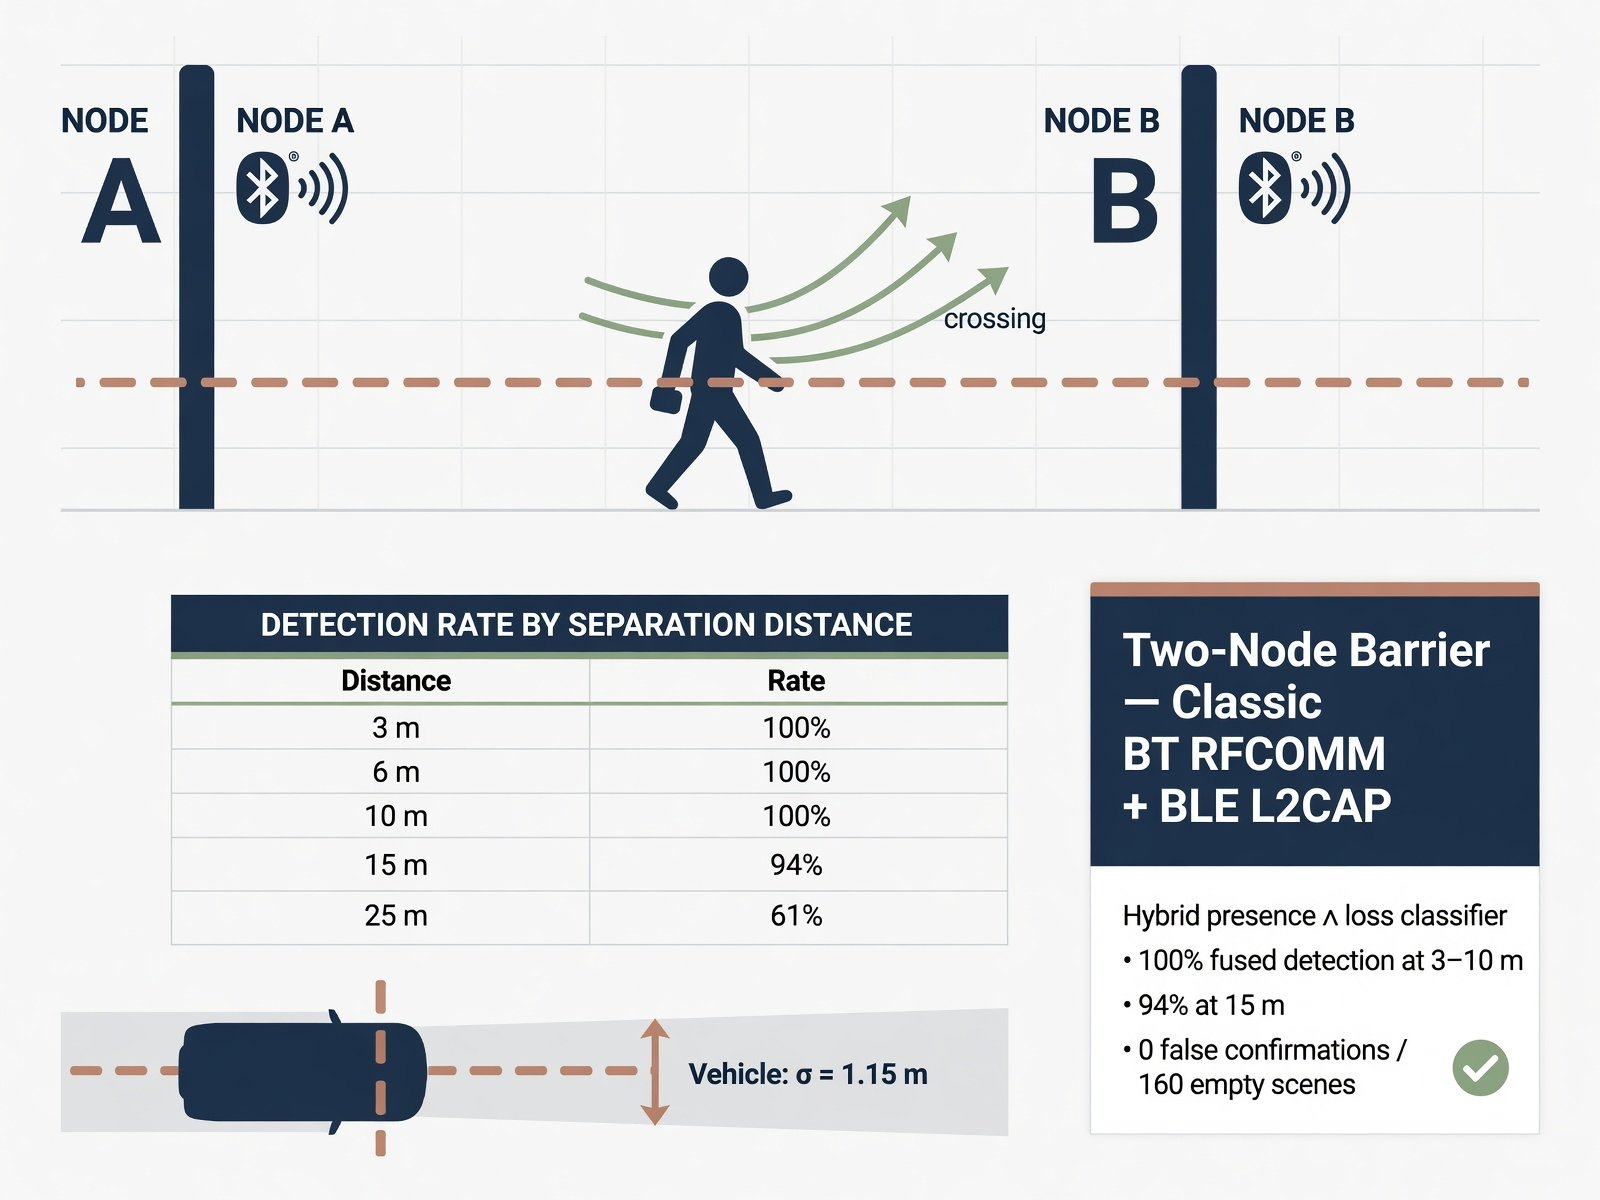
\includegraphics[width=8.7cm]{fig_modern_06_transit.jpg}
  \caption{The \emph{Transit} tab: a two-node barrier over Classic Bluetooth
  RFCOMM and BLE L2CAP; both a link drop and a link appearance are treated as
  evidence, and detection is reported at each separation. The rate panel is
  the app's displayed summary (its 15\,m value is the BLE channel, its 25\,m
  value the hybrid); measured per-channel rates with confidence intervals are
  in Section~V-G.}
  \label{fig:transit}
\end{figure}


%---------------------------------------------------------------------------
% VI. DISCUSSION
%---------------------------------------------------------------------------
\section{Discussion}
The field envelope narrows beyond 12\,m: detection falls from 73.3\,\% at 8\,m to 50.0\,\% at 16\,m and
15.0\,\% at 22\,m, while the observed dip depths approach the adaptive trigger
floor in the same interval, exactly the behaviour Eq.~\eqref{eq:pathloss} anticipates when
scintillation begins to dominate the shadow term. Two platform effects shape
the measured curve. First, Android 15 BLE scan throttling reduces the
effective sample rate at distances where the dip margin is thin; the
foreground-service configuration mitigates but cannot remove the duty cycle.
Second, vehicle transits at road speed compress dip duration toward the
detector gate, which explains why vehicle detection sits below pedestrian
detection at 8--16\,m despite the wider vehicle profile. Both effects are
properties of the deployed platform and traffic, not of the radio model, and
both argue for reporting distance-conditioned rates rather than a single
accuracy figure.

\textbf{Roles of the mesh and gamification.} The mesh turns a bounded
single-device sensor into a collective one: cross-node agreement within the
stated tolerances confirms events where single-link evidence is weakest,
overlapping envelopes tile wider areas, and the reliability bonus steers
nodes toward informative geometries. Gamification sustains the participation
this collective sensor depends on.

\textbf{Scope of the validation.} This campaign validates the single-device
sensing stack---detection, classification, vehicle detection, gated ranging, epoch
change detection, silent-control false positives, and the displayed accuracy
estimate---together with the two-node transit counter, including direction
estimation and end-to-end false confirmations (Section~V-G). The cooperative
mesh (Section~II-D) is exercised here only as a deployed interface; its
confirmation and false-confirmation performance requires a distributed
multi-node campaign and is left to future work, as is gamification behaviour
under sustained multi-user participation.

\textbf{Threats to validity.} (1)~Single device, single site:
generalisability to other phones and environments is unquantified.
(2)~Open car park: the multipath environment is simpler than urban canyons;
performance may degrade further. (3)~Ground-truth timing: manual counters
introduce $\pm1$\,s uncertainty, which affects per-event classification more than
aggregate counts. (4)~Sample size: $n = 15$--$20$ per cell gives wide
confidence intervals at low detection rates; larger batteries of crossings
are planned. (5)~Weather and traffic were not stratified; sessions span dry
daytime conditions only.

%---------------------------------------------------------------------------
% VII. CONCLUSIONS
%---------------------------------------------------------------------------
\section{Conclusions and Future Work}
MeshCrowd demonstrates that commodity smartphones can form a practical,
infrastructure-free sensing platform by combining BLE and dual-band Wi-Fi
measurements for passive multi-band detection, gated ranging, field-change
detection, two-node transit counting, and cooperative mesh sensing, and this
paper reports the first complete physical validation of the single-device
stack on an unmodified handset. In the field, a single phone detects
pedestrian crossings to about 16\,m (50\,\%) and sustains classification above 80\,\% inside 6\,m, detects moving vehicles to 16\,m at reduced rate, holds a
zero-BLE-false-positive budget over 30\,h of silent control, and refuses
range estimates exactly where the measured signal cannot support them. The
resulting architecture supports applications ranging from \textbf{two-node
pedestrian and vehicle counting} at entrances and corridors, to \textbf{urban
crowd and flow monitoring}, \textbf{smart-mobility and roadside awareness},
and \textbf{emergency situational awareness} where dedicated sensing
infrastructure is unavailable, with a gamification layer linking
participation and rewards to measurement agreement.

Future evaluation will focus on the distributed multi-device campaign that
this campaign deliberately excludes: mesh confirmation and
false-confirmation rates across node densities, and gamification dynamics
under sustained participation, alongside diverse indoor and outdoor
environments, device heterogeneity, placement, multipath, interference, and
battery constraints. Mesh resilience against spoofed or adversarial reports
also remains untested; future work will address \textbf{mesh integrity and
incentive robustness}, extending the current agreement-based rewards toward
reputation- and quality-aware mechanisms that remain reliable under noisy,
spoofed, or coordinated device behavior.

%---------------------------------------------------------------------------
% References
%---------------------------------------------------------------------------
\balance
\begin{thebibliography}{26}

\bibitem{wilson2010} J.~Wilson and N.~Patwari, ``Radio tomographic imaging with
wireless networks,'' \emph{IEEE Trans.\ Mobile Comput.}, vol.~9, no.~5,
pp.~621--632, May 2010, doi: 10.1109/TMC.2010.8.

\bibitem{januszkiewicz2018} {\L}.\,Januszkiewicz, ``Analysis of human body
shadowing effect on wireless sensor networks operating in the 2.4~GHz band,''
\emph{Sensors}, vol.~18, no.~10, art.~3412, Oct. 2018, doi:
10.3390/s18103412.

\bibitem{alippi2016} C.~Alippi, M.~Bocca, G.~Boracchi, N.~Patwari, and
M.~Roveri, ``RTI goes wild: Radio tomographic imaging for outdoor people
detection and localization,'' \emph{IEEE Trans.\ Mobile Comput.}, vol.~15,
no.~10, pp.~2585--2598, Oct. 2016, doi: 10.1109/TMC.2015.2504964.

\bibitem{li2024} Z.~Li, A.~Dubey, S.~Shen, N.~K.~Kundu, J.~Rao, and R.~Murch,
``Radio tomographic imaging with reconfigurable intelligent surfaces for
integrated sensing and communication,'' \emph{IEEE Trans.\ Wireless Commun.},
vol.~23, no.~11, pp.~15784--15797, Nov. 2024, doi: 10.1109/TWC.2024.3433011.

\bibitem{wu2024} H.~Wu, C.~Cheng, C.~Peng, T.~Zhou, and T.~Chen, ``Combining
transformer with a latent variable model for radio tomography based robust
device-free localization,'' \emph{Comput.\ Commun.}, vol.~224, art.~108022,
Oct. 2024, doi: 10.1016/j.comcom.2024.108022.

\bibitem{wong2024} W.~E.~Wong, A.~H.~Wong, W.~Q.~Peh, and C.~K.~Tan, ``A
high-dimensional, multi-transceiver channel state information dataset for
human activity recognition,'' \emph{Data Brief}, vol.~55,
art.~110673, Aug. 2024, doi: 10.1016/j.dib.2024.110673.

\bibitem{sanchez2020} D.~S\'anchez-Rodr\'iguez, M.~A.~Quintana-Su\'arez,
I.~Alonso-Gonz\'alez, C.~Ley-Bosch, and J.~J.~S\'anchez-Medina, ``Fusion of
channel state information and received signal strength for indoor localization
using a single access point,'' \emph{Remote Sens.}, vol.~12, no.~12,
art.~1995, Jun. 2020, doi: 10.3390/rs12121995.

\bibitem{ramirez2021} R.~Ramirez, C.-Y.~Huang, C.-A.~Liao, P.-T.~Lin, H.-W.~Lin,
and S.-H.~Liang, ``A practice of BLE RSSI measurement for indoor positioning,''
\emph{Sensors}, vol.~21, no.~15, art.~5181, Jul. 2021, doi: 10.3390/s21155181.

\bibitem{milano2024} F.~Milano, H.~da Rocha, M.~Larocca, L.~Ferrigno,
A.~Esp\'iritu Santo, J.~Salvado, and V.~Paciello, ``BLE-based indoor
localization: Analysis of some solutions for performance improvement,''
\emph{Sensors}, vol.~24, no.~2, art.~376, Jan. 2024, doi: 10.3390/s24020376.

\bibitem{bai2020} L.~Bai, F.~Ciravegna, R.~Bond, and M.~Mulvenna, ``A low cost
indoor positioning system based on Bluetooth Low Energy,'' \emph{IEEE Access},
vol.~8, pp.~136858--136871, 2020, doi: 10.1109/ACCESS.2020.3012342.

\bibitem{khan2023} D.~Khan and I.~W.-H.~Ho, ``CrossCount: Efficient device-free
crowd counting by leveraging transfer learning,'' \emph{IEEE Internet Things
J.}, vol.~10, no.~5, pp.~4049--4058, Mar. 2023.

\bibitem{zhou2020} R.~Zhou, Z.~Gong, X.~Lu, and Y.~Fu, ``WiFlowCount:
Device-free people flow counting by exploiting Doppler effect in commodity
WiFi,'' \emph{IEEE Syst.\ J.}, vol.~14, no.~4, pp.~4919--4930, Dec. 2020.

\bibitem{zhang2022} J.~Zhang, X.~Li, S.~Shi, \emph{et al.}, ``A reputation-based
and privacy-preserving incentive scheme for mobile crowd sensing: A deep
reinforcement learning approach,'' \emph{Wirel.\ Netw.}, 2023, doi:
10.1007/s11276-022-03111-9.

\bibitem{wang2018} J.~Wang, M.~Li, Y.~He, H.~Li, X.~Xiao, and C.~Wang, ``A
blockchain based privacy-preserving incentive mechanism in crowdsensing
applications,'' \emph{IEEE Access}, vol.~6, pp.~17545--17556, 2018, doi:
10.1109/ACCESS.2018.2815365.

\bibitem{casar2022} M.~C\"asar, T.~Pawelke, J.~Steffan, and G.~Terhorst, ``A
survey on Bluetooth Low Energy security and privacy,'' \emph{Comput.\ Netw.},
vol.~202, art.~108712, Jan. 2022, doi: 10.1016/j.comnet.2021.108712.

\bibitem{antonioli2020} D.~Antonioli, N.~O.~Tippenhauer, and K.~B.~Rasmussen,
``Key negotiation downgrade attacks on Bluetooth and Bluetooth Low Energy,''
\emph{ACM Trans.\ Priv.\ Secur.}, vol.~23, no.~3, art.~14, Jul. 2020, doi:
10.1145/3394497.

\bibitem{cai2024} H.~Cai, ``Securing billion Bluetooth devices leveraging
learning-based techniques,'' in \emph{Proc.\ AAAI Conf.\ Artif.\ Intell.\
(AAAI)}, vol.~38, no.~21, pp.~23731--23732, 2024, doi:
10.1609/aaai.v38i21.30544.

\bibitem{Brown2001Wilson} L.~D.~Brown, T.~T.~Cai, and A.~DasGupta, ``Interval
estimation for a binomial proportion,'' \emph{Statist.\ Sci.}, vol.~16, no.~2,
pp.~101--133, 2001, doi: 10.1214/ss/1009293286.

\bibitem{Hanley1983RuleOfThree} J.~A.~Hanley and A.~Lippman-Hand, ``If nothing
goes wrong, is everything all right? Interpreting zero numerators,''
\emph{JAMA}, vol.~249, no.~13, pp.~1743--1745, 1983, doi:
10.1001/jama.1983.03330370053030.

\bibitem{patwari2010proc} N.~Patwari and J.~Wilson, ``RF sensor networks for device-free localization: Measurements, models, and algorithms,'' \emph{Proc. IEEE}, vol.~98, no.~11, pp.~1961--1973, Nov.~2010, doi: 10.1109/JPROC.2010.2079090.
\bibitem{wilson2011} J.~Wilson and N.~Patwari, ``See-through walls: Motion tracking using variance-based radio tomography networks,'' \emph{IEEE Trans. Mobile Comput.}, vol.~10, no.~5, pp.~632--643, May 2011.
\bibitem{wang2015har} W.~Wang, A.~X.~Liu, M.~Shahzad, K.~Ling, and S.~Lu, ``Understanding and modeling of WiFi signal based human activity recognition,'' in \emph{Proc. 21st Annu. Int. Conf. Mobile Comput. Netw. (MobiCom)}, 2015, pp.~65--76.
\bibitem{ma2019wifi} Y.~Ma, G.~Zhou, and S.~Wang, ``WiFi sensing with channel state information: A survey,'' \emph{ACM Comput. Surv.}, vol.~52, no.~3, art.~47, 2019, doi: 10.1145/3310194.
\bibitem{ryan2013woot} M.~Ryan, ``Bluetooth: With low energy comes low security,'' in \emph{Proc. 7th USENIX Workshop on Offensive Technologies (WOOT)}, 2013.
\bibitem{beresford2003} A.~R.~Beresford and F.~Stajano, ``Location privacy in pervasive computing,'' \emph{IEEE Pervasive Comput.}, vol.~2, no.~1, pp.~46--55, Jan.--Mar. 2003.
\bibitem{herrera2010} J.~C.~Herrera, D.~B.~Work, R.~Herring, X.~J.~Ban, Q.~Jacobson, and A.~M.~Bayen, ``Evaluation of traffic data obtained via GPS-enabled mobile phones: The Mobile Century field experiment,'' \emph{Transp. Res. Part C: Emerg. Technol.}, vol.~18, no.~4, pp.~568--583, Aug. 2010.
\end{thebibliography}

\end{document}
